% ==================== PART 1 — Auto research result (agent-written) ====================
% Reframed (write-vs-train regime). Fig 1 = figs/fig1.pdf (result); Fig 2 = figs/pipeline.pdf (method).
% "Our tester" = the loop's champion (headline) program; "the loop's programs" = the class. NO per-task max is taken.

\section{Introduction}
\label{sec:intro}
Automated game testing needs an \emph{exploration} policy that drives a game into the rare states that trigger a planted
defect or satisfy a level's win condition, and reaches them within the small interaction budget a QA pass can afford. The
reflex is to \textbf{train} a reinforcement-learning (RL) explorer, usually PPO with an intrinsic-motivation bonus, once
per game. But trained RL is costly in interaction, needs per-game reward shaping and tuning, and transfers poorly, so at a
tester's real budget it under-explores.

We take the opposite route. Rather than \textbf{train} a policy, an autonomous LLM-evolution loop \textbf{writes} an
exploration \emph{program} and evolves it: over many generations a proposal LLM writes and mutates candidate procedures,
and a multi-engine fitness keeps the ones that reach the most target states at a fixed budget, with every counted hit
replayed from a clean reset~\citep{funsearch}. Our central finding is a sharp, budget-matched boundary:
\textbf{at an equal interaction budget, on sparse-reward target-reaching, a single zero-training program the loop wrote
out-reaches a tuned RL explorer and every baseline; given $4$--$16\times$ more interaction, or on reward-dense tasks,
training catches up.} Writing and training the tester are not rivals but regimes, split by reward density and budget, and
the loop maps that split cheaply. To our knowledge this is the first budget-matched demonstration that a written
exploration program out-reaches trained RL for game testing, with every counted result execution-verified.

\textbf{Contributions.} (i) A loop that discovers game-testing exploration \emph{programs}, and the map of where a written
program beats a trained one. (ii) The headline (Fig.~\ref{fig:main}): on four sparse-reward tasks across three engines, our
tester is the single best method at equal budget, above random, action-repeat, plain Go-Explore, and tuned PPO. The win is
the discovered strategy, not the archive, and it transfers to engines the search never saw. (iii) A verification backbone,
replay-from-reset of every counted hit over a frozen hashed protocol with sealed splits and a reachability calibration,
which caught the loop inflating its own fitness (\S\ref{sec:setup}, Part~2). The programs, the benchmark, and this Part
were produced by the loop. We do not overclaim universality: our tester ties two saturated tasks a trivial baseline also
wins, cedes reward-dense Craftax to PPO, and does not yet run at Kinetix protocol scale. We draw that map in full.

\section{Related work}
\label{sec:related}
\textbf{RL exploration / PPO.} Count-based~\citep{tang2017}, RND~\citep{rnd}, and ICM~\citep{icm} augment a trained
policy's reward to seek novelty; they need $10^6$--$10^8$ steps to warm up, so at a tester's budget the bonus is cold.
\emph{We match the budget and train nothing.}
\textbf{Go-Explore / archive methods.} Go-Explore~\citep{goexplore} keeps an archive of returnable states and is the
strongest classical family, but its wins hinge on a hand-chosen cell abstraction and are shown per game. \emph{We show a
plain archive is not enough, since the win is the discovered strategy over it, and evaluate across engines.}
\textbf{Action-repeat.} A stochasticity control~\citep{machado2018}, not an exploration method. \emph{We include it as a
baseline; it is our tightest competitor on physics and our weakest on navigation.}
\textbf{LLMs that write code for control.} FunSearch~\citep{funsearch} evolves programs; Eureka~\citep{eureka} writes
rewards and trains RL; PromptPO~\citep{promptpo} writes control policies for return; TITAN~\citep{titan} runs a per-step LLM
agent as a tester. \emph{We occupy the point they leave open: budget-matched, target-reaching, and replay-verified, a
written exploration program that is paid once and run training-free.} Table~\ref{tab:caps} places the families on the axes
that matter.

\begin{table}[t]\centering\small
\caption{Where each family sits. Our tester is the one that is budget-matched, training-free, and target-reaching at
once; universality across all tasks is \emph{not} claimed (\S\ref{sec:result}).}
\label{tab:caps}
\begin{tabular}{@{}lcccc@{}}\toprule
 & no per-env & fixed interaction & sparse-reward & replay-\\
 & training & budget & target-reaching & verified \\ \midrule
PPO + intrinsic~\citep{tang2017,rnd,icm} & \ding{55} & \ding{55} & partial & \ding{55} \\
Go-Explore~\citep{goexplore} & \checkmark & partial & \checkmark & \ding{55} \\
Action-repeat~\citep{machado2018} & \checkmark & \checkmark & \ding{55} & \ding{55} \\
Eureka / PromptPO~\citep{eureka,promptpo} & \ding{55}/\checkmark & \ding{55} & \ding{55} & \ding{55} \\
\textbf{Written program (ours)} & \checkmark & \checkmark & \checkmark & \checkmark \\ \bottomrule
\end{tabular}
\end{table}

\section{The result}
\label{sec:result}
\begin{figure*}[t]\centering
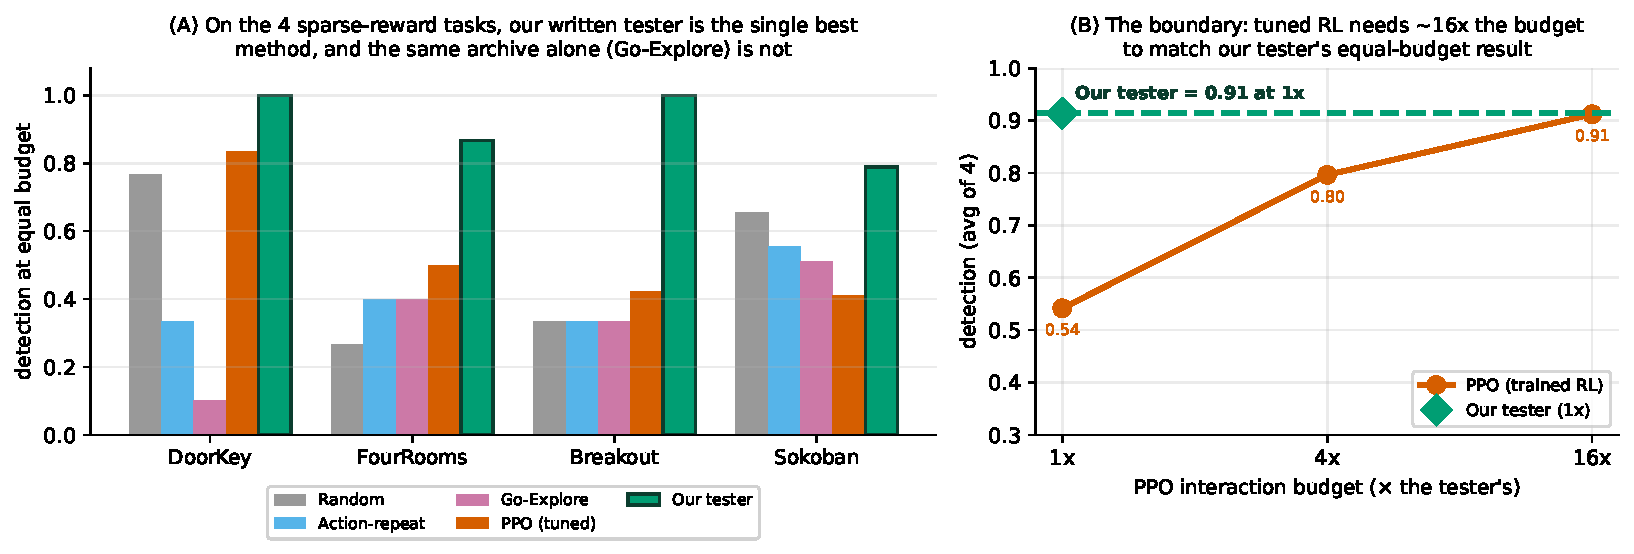
\includegraphics[width=\textwidth]{figs/fig1.pdf}
\caption{\textbf{(A)} At an equal interaction budget on the four sparse-reward tasks, our tester is the single best method,
above random, action-repeat, plain Go-Explore (the \emph{same} save/restore archive), and tuned PPO. Go-Explore's $0.10$ on
DoorKey shows the win is the discovered strategy, not the archive. \textbf{(B)} The boundary: only PPO's budget scales, and
tuned PPO needs about $16\times$ the interaction to match our tester's $1\times$ result (PPO is best-of-3 objectives at
$4/16\times$).}
\label{fig:main}
\end{figure*}

\textbf{The equal-budget win (Fig.~\ref{fig:main}A).} We report one program, unchanged across tasks, reaching on average
$0.91$ of the targets against $0.54$ for tuned PPO. Per task it beats every baseline at equal budget: DoorKey $1.00$,
FourRooms $0.87$, Breakout $1.00$, Sokoban $0.79$, against tuned PPO $0.83/0.50/0.42/0.41$, action-repeat
$0.33/0.40/0.33/0.56$, Go-Explore $0.10/0.40/0.33/0.51$, and random $0.77/0.27/0.33/0.66$. These are the sparse-reward,
non-saturated tasks in the suite, chosen along one axis, reward density; on them, winning requires real exploration that no
cheap baseline provides. Our tester's full record on every task, including where it ties or loses, is the map below.

\textbf{The boundary is the thesis (Fig.~\ref{fig:main}B).} The claim is strictly equal-budget. Scaling only PPO's budget,
its average climbs from $0.54$ at $1\times$ to $0.91$ at $16\times$, matching what our tester reaches at $1\times$; PPO
overtakes our tester on DoorKey at $4\times$ and on Breakout and Sokoban at $16\times$. We explicitly withdraw any ``RL
never catches up'' reading: it does, given an order of magnitude more interaction. That split is the contribution. Write
once and win at the tester's budget, or train and win with a larger one.

\textbf{Strategy, not archive; and it transfers.} Plain Go-Explore has the \emph{same} archive yet scores $0.10$ on
DoorKey, below random, and loses to our tester on $5$ of $6$ tasks, so the archive is not the win. And the win transfers
across engines: our tester was evolved once on a multi-engine fitness (Kinetix, Craftax, and Gymnax) that never saw
MiniGrid, MinAtar, or Sokoban, while a \emph{fresh} DoorKey-only search reaches just $0.33$ (beating Go-Explore, losing to
transfer). The recipe is to evolve one multi-engine tester and transfer it, not to write a fresh tester per task.

\textbf{The map (where a written program does \emph{not} win).} Our tester's full row: on MountainCar and DeepSea-24 it
scores $1.00$, but so does trivial action-repeat, so these are ceiling ties with no exploration skill on display (excluded
from the claim above); on reward-dense \textbf{Craftax it loses}, $0.27$ against PPO $0.34$; and it does not run at Kinetix
protocol scale, a compile-time limit of its archive that sibling programs cover (\S\ref{sec:setup}). This is the regime
boundary: writing wins where reward is sparse and the budget is tight; on our one reward-dense task and at $4$--$16\times$
the budget, training wins.

\section{Setup and the verification backbone}
\label{sec:setup}
\textbf{Testers as programs} (Fig.~\ref{fig:pipeline}). A tester is four pure-JAX hooks
(\texttt{init/restore/act/archive}) over an archive of save/restore-able states, run as $B$ workers for $T$ steps, so the
budget is $B\!\cdot\!T$; the same interface runs on every engine through a generic feature head. PPO is trained on the
\emph{same} feature head, with no observation handicap, and its training steps \emph{are} its budget. The equal-budget PPO
column (Fig.~\ref{fig:main}A) is best over a $5$-objective sweep (count, RND, ICM, proximity-curiosity, and task reward)
crossed with \{default, tuned $lr{=}10^{-4}$, $\text{ent}{=}0.2$\}; the crossover curves (Fig.~\ref{fig:main}B) are
best-of-$3$ objectives, labeled as such. Testers use $5$ seeds and PPO $3$ to $5$; we report one fixed program.

\begin{figure}[t]\centering
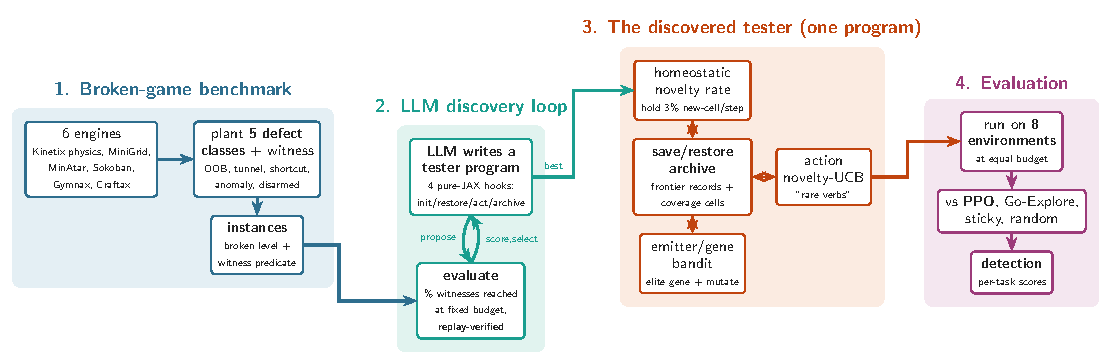
\includegraphics[width=\linewidth]{figs/pipeline.pdf}
\caption{The loop: break six engines into defect classes with programmatic witnesses; an LLM writes and mutates tester
programs scored on a multi-engine fitness (Kinetix hits replayed from reset, \S\ref{sec:setup}); the single champion
program explores through a save/restore archive driven by three runtime modules; evaluate against PPO, Go-Explore,
action-repeat, and random at equal budget.}
\label{fig:pipeline}
\end{figure}

\textbf{Depth and verification (Kinetix planted defects).} The rigor lives here. We plant five defect classes
(\textsc{oob}, \textsc{tunnel}, i.e.\ clipping, \textsc{shortcut}, \textsc{anomaly}, \textsc{disarmed}) with programmatic
witness predicates over $74$ shipped and $64$ generated levels, and \textbf{every counted hit is re-simulated from a clean
level reset and must re-raise the witness, or it is a miss}. The protocol is frozen and hashed; a $30\%$ level split and a
whole defect class are sealed from the search, and a reachability calibration bounds what any tester can witness. The
loop's strongest Kinetix program (a sibling of our tester, which does not run at this scale) leads a large method field on
the search split ($0.655$ against action-repeat $0.602$, PPO $0.566$, random $0.494$), but that is \emph{in-sample}
selection, and on held-out levels its lead over action-repeat narrows to a near-tie, so we headline the apparatus rather
than the search-split margin. Part~2 recounts how this apparatus caught the loop inflating its own fitness by $+0.11$
through a harness race, the check the whole result rests on.

\section{Limitations}
\label{sec:limits}
The claim is equal-budget on sparse-reward target-reaching; given $4$--$16\times$ more interaction, tuned PPO catches up
(Fig.~\ref{fig:main}B), and action-repeat is a close competitor on Kinetix \emph{physics}. Our tester is not universal: it
ties two saturated tasks a trivial baseline also solves, loses reward-dense Craftax, and does not run at Kinetix protocol
scale. It uses a save/restore archive a learned policy cannot, a legitimate strategy difference (archive-based program
against learned policy at equal budget, the comparison the Go-Explore/RL literature already makes), which we control for
with identical features and a plain-archive baseline. Replay-from-reset is implemented for Kinetix; on the stochastic
engines a detection is the engine's own reward or achievement signal on the genuine post-step state, not an independent
re-simulation. Kinetix is a research substrate, not a shipped game. Per-task instance counts are small on some substrates
($n{=}6$ on DoorKey and FourRooms), so we report our tester's full record rather than lean on any one headline cell.
